

The first goal of the proposed work is to further develop the Fusion Browser prototype described in \Cref{chap:fusion} for a public field deployment and test the entity-centric approach in real-life settings. Based on lab studies and talking with participants afterwards, I have identified two areas where the current system can be improved and extended to cover user needs that are currently unsupported: capturing structured information about entity such as attributes or opinions and organizing collected information more flexibly to reflect their evolving mental models. Addressing these has the potential of allowing the system to better supporting the next steps in online sensemaking -- structuring information and supporting decision-making.

My primary focus will be on further developing the research prototype that focused on information foraging for a public release while experimenting with new approaches within the same system to support structuring and decision-making. While a public deployment has the potential of allowing the system to reach a wider audience outside of the lab and collect usage information at scale, user tests and lab studies may also be required throughout the process of design and development.
Success in gaining popularity would also depend on many factors outside of the scope of my dissertation, such includes visual design, marketing and market understanding, and competing commercial products. While the aim is to develop a large user-base, the proposed approaches can also be evaluated with lab studies and smaller scale field deployments using participants recruited from a local participant pool (CBDR). 

\begin{figure}
\centering
\begin{minipage}{.49\textwidth}
  \centering
  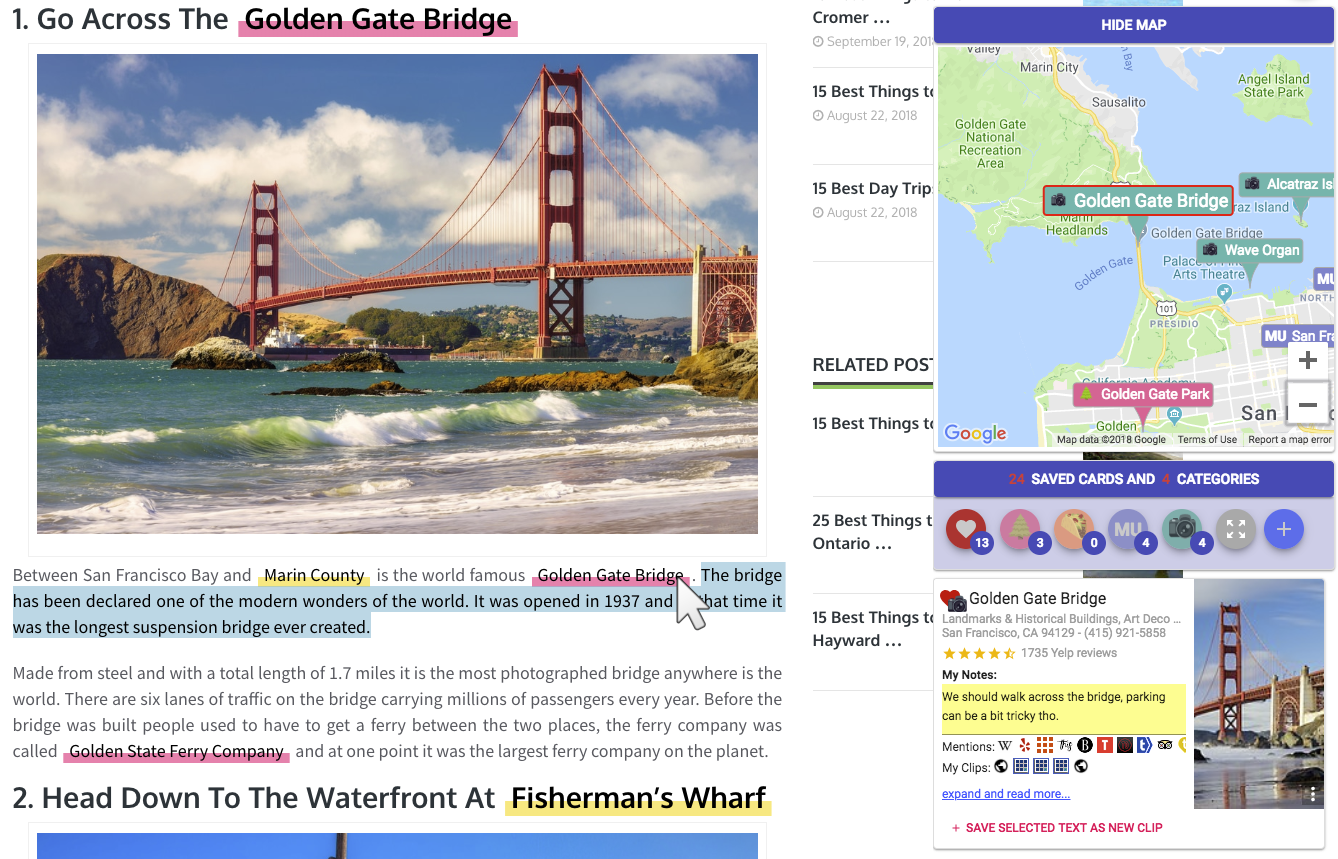
\includegraphics[width=\textwidth]{Chapters/Fusion/main.png}
\end{minipage}%
\begin{minipage}{.49\textwidth}
  \centering
  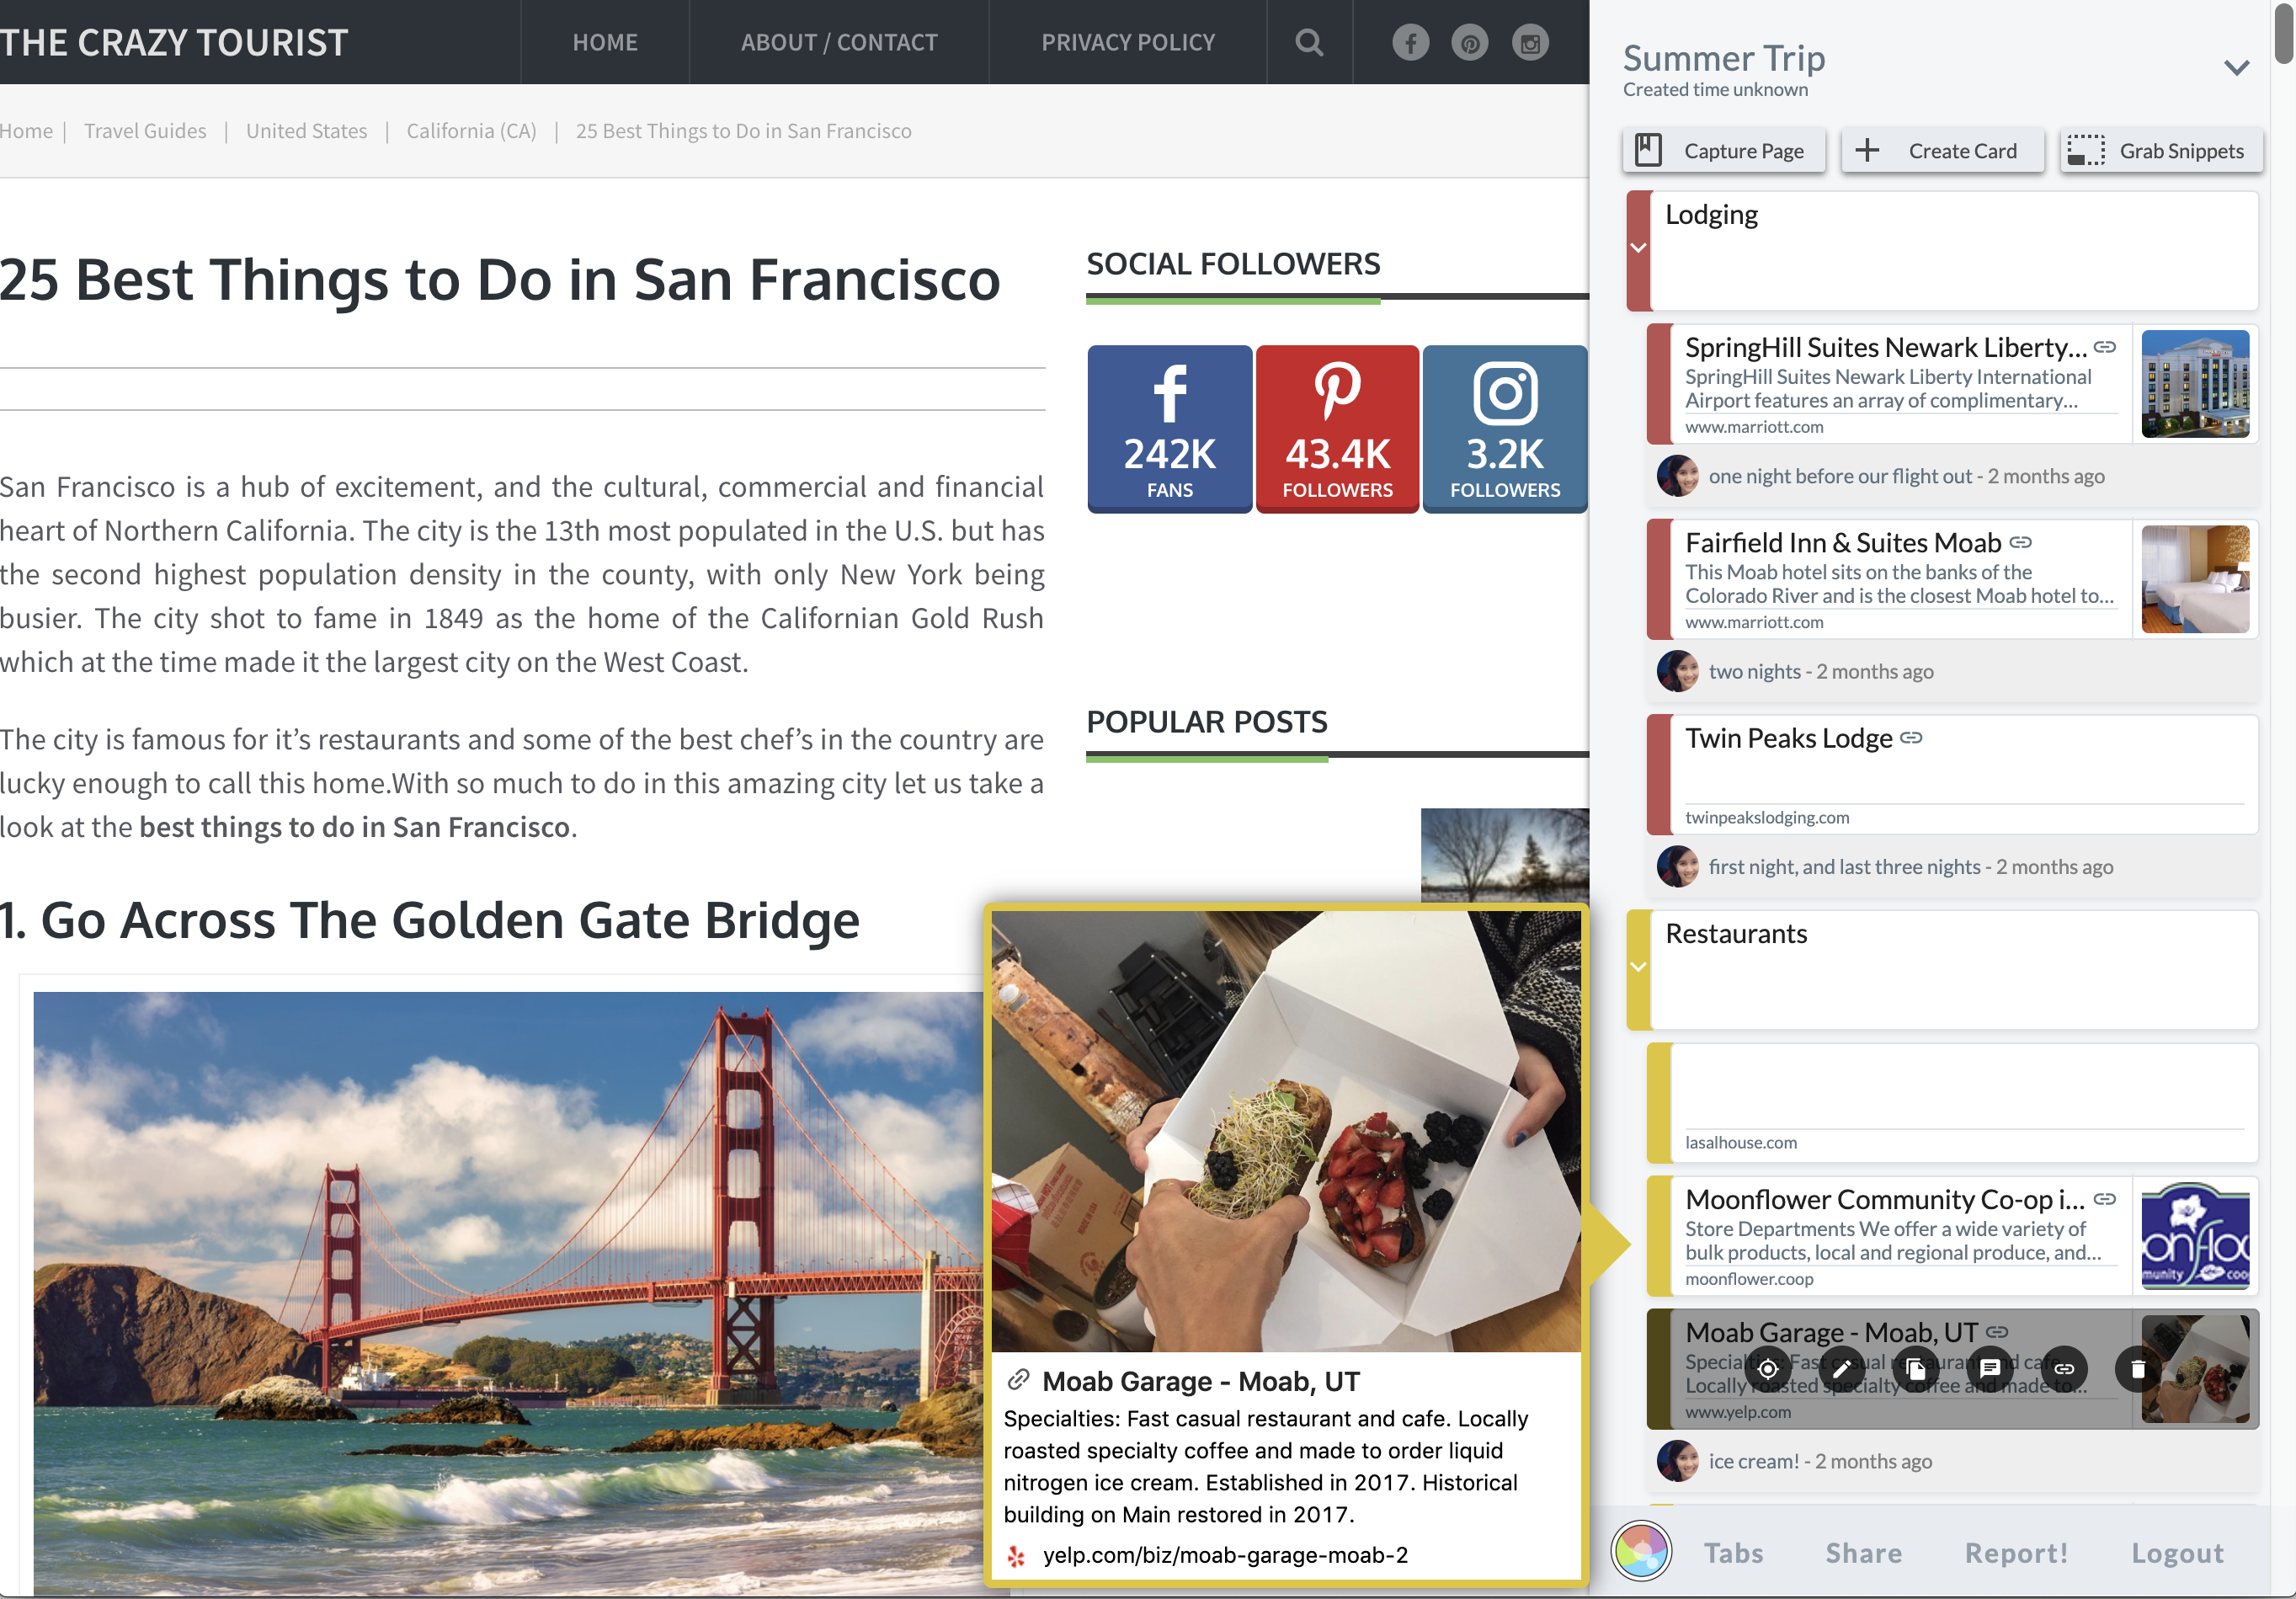
\includegraphics[width=\textwidth]{images/fuse.png}
\end{minipage}
\caption{The current prototype allowed users to access entity cards generated by the system, and saved on into categories (left). In the new design, users can also create notes and category cards, and nest cards to create a hierarchy structure (right).}
\label{fig:test2}
\end{figure}

\section{Structuring Collected Inforamtion}

In \Cref{chap:fusion} I presented a prototype system called Fusion Browser that focused on exploiting common entities mentioned across webpages in a complex search task as a substrate to support foraging. One the features of Fusion Browser is to allow users to save information about an entity to be propagated and resurfaced across other webpages that also mentioned the same entity, allowing users to efficiently cross-reference and build on their prior effort as they explore more webpages. While participants generally agreed that this entity-centric approach lowered the cost of foraging during complex search tasks, they also pointed to its limitations. Specifically, the current prototype only allowed users to attach information to entity cards and organize cards under categories. While participants found this to be effective for foraging, they also expressed needs for more flexible structures to better support decision-making. They cited their current practices of using word processors (such as Google Docs) to create outlines or tables containing both information copied from webpages and manual notes about their own thoughts and decisions.

Due to its ubiquity and generalizability, I plan to extend the current prototype to support building outlines during foraging. In the new design, instead of attaching collected information to entity cards created by the system, users can freely create manual note cards to externalize their thoughts and decisions. To create structures that can better reflect users' mental models, in the new design users can also nest cards under other cards to create hierarchies. This design is similar to how many participants reported using note taking software during complex search tasks, but the core challenge here is to lower the cost of structuring and externalization as they can be either disruptive for users' reading process or prohibitive for externalizing \cite{o1996towards,marshall1999introducing,tashman2011liquidtext,bianchi2015designing}. My insights from developing Fusion Browser (\Cref{chap:fusion}) that focused on in-situ information foraging represent a unique starting point for investigating ways to support in-situ information structuring as users explore and foraging from multiple webpages in a complex search task. In addition, my past work on the Alloy system (\Cref{chap:alloy}) for structuring web content with machine learning and crowd-microtasks can also provide insights on designs and interactions that can further lower the costs of structuring for the end users through machine learning.

\section{Structuring Entity Options}

The current prototype as presented in \Cref{chap:fusion} identified entities mentioned in the webpages a user read and enriched their browsing experience with rich entity cards with attributes from external knowledge bases. For example, showing reviews, ratings and locations of different attractions in a travel task or showing the weight and resolution of different cameras in a shopping task. In the current prototype we arbitrarily surfaced 
While knowledge bases such as DBpedia \cite{dbpedia} typically have dozens to hundreds of attributes for a single entity, the current prototype in \Cref{chap:fusion} only surfaced a few common attribute types I considered the most useful and were hard coded into the system so it does not overwhelm users (e.g., location, short description, and categories.) Participants in general found the attributes Fusion presented to be useful, but also pointed to scenarios where they wished to create more fine-grained attribute to compare their options. These can break down into two main categories described below.

Firstly, participants wanted to capture additional attributes that were missing in the entity cards. One example would be to update the address of a restaurant that was outdated in or missing in external knowledge sources. Another was to access attributes information that were actually available in external knowledge sources but not surfaced by the current prototype, such as the weights and the sensor sizes of different camera models they were comparing.
More fundamentally, participants also relied on soft and/or subjective criteria from exploring reviews and online recommendations to make predictions about how well different options might match their personal interests and needs. While the current current prototype allowed users to capture such subjective attributes as collections of notes and clips associated with different entities, it can be difficult to compare multiple entities such as manually compiling a comparison table.

The core challenge here is that in early stages, users often do not yet know the attributes important to their own needs, and have to gradually discover them through exploration in order to make an decision. For example, a camera shopper might discover from a tutorial that sensor size is an important factor for taking photos at night, or a traveler might discover the different styles of ramen broth while an in-depth review.
This need for was also highlighted in my work in \Cref{chap:searchlens} on assisting users in developing and externalizing their nuanced interests while searching reviews and in  \Cref{chap:highlight} for supporting uncertainty while saving information in early stages of exploratory searches. Building on insights from these work, I plan to extend the current prototype to support users in developing and externalizing nuanced interests and criteria during foraging, and allow them to structure entity options that they have collected for comparison.

\section{Evaluation and Contributions}

%I plan to conduct studies to explore this idea in two phases: First, a controlled lab study focusing on how this entity-centric approach can benefit foraging across webpages. I will use the findings from study 1 to inform the development and public release of a browser extension that supports both entity-centric foraging and structuring.

%For Study 1, I will build a prototype system for a controlled lab study to explore the benefits and challenges of the entity-centric approach for reading, cross-referencing, and collecting information across multiple webpages in the browser. I plan to explore whether the gather- and propagate-based features can allow participants to cross-reference and re-access previously saved notes efficiently and whether participants consider having the additional features an improvement to their current methods.
Since note taking and structuring are longer term activities when compared to foraging, I plan to publically release a browser extension for Chrome to reach a wider audience, collect usage information. This would allow me to gather quantitative data based on real-life tasks, for example: 

\begin{itemize}
    \item Time spent using the system
    \item Types of tasks conducted
    \item Features utilized
    \item Number of different types of cards created per task
    \item Number of attributes captured per task
\end{itemize}

Throughout development, I will also conduct lab studies and usability tests to collect qualitative data and better understand how users may utilize the system, for example:

\begin{itemize}
    \item General usability of the system
    \item Whether decisions were made using the system, and how the system supported the decision making process
    \item Confidence in their process and decision
    \item Overall preferences, satisfaction and motivation
\end{itemize}

The core contribution of the proposed work is an entity-centric approach for supporting sensemaking across webpages in the browser when conducting complex exploratory search tasks, which includes:

\begin{itemize}
\item An extension that enables the browser to better understand the content of webpages by identifying entities using existing natural language processing algorithms and external knowledge sources (e.g., Wikipedia and Yelp), lowering the cost of cross-referencing different entities across webpages, searches, and external knowledge sources. 
\item A context-aware workspace where users can easily gather and structure options and evidence across multiple webpages, where relevant information saved previously will be resurfaced by the system as users browse different pages.
\end{itemize}

Equipping browsers and note-taking interfaces the ability to identify and connect options and evidence scattered across tabs and personal notes have the potentials of lowering the efforts required to make sense of and forage from many information sources. Empowering users to capture, associate, and structure fluidly their findings as they read and understand more information. Successes in doing so may also lead to useful insights on the design of future intelligent browser interfaces that can better understand the information being consumed by its users, and building novel interactive systems for supporting online sensemaking.


\section{Timeline and Submission Plans}

\subsection*{Timeline}

\begin{itemize}
    \item April - June 2019: Prototype Development
    \item June - August 2019: Deployment
    \item August - September 2019: Evaluation and Analysis
    \item October - December 2019: Write Dissertation and Defend 
\end{itemize}

\subsection*{Submission Plans}

\begin{itemize}
    \item ACM UIST 2019: \Cref{chap:fusion}
    \item ACM SIGCHI 2019: \Cref{chap:proposed}
\end{itemize}